\let\negmedspace\undefined
\let\negthickspace\undefined
\documentclass[journal]{IEEEtran}
\usepackage[a5paper, margin=10mm, onecolumn]{geometry}
%\usepackage{lmodern} % Ensure lmodern is loaded for pdflatex
\usepackage{tfrupee} % Include tfrupee package

\setlength{\headheight}{1cm} % Set the height of the header box
\setlength{\headsep}{0mm}     % Set the distance between the header box and the top of the text

\usepackage{gvv-book}
\usepackage{gvv}
\usepackage{cite}
\usepackage{amsmath,amssymb,amsfonts,amsthm}
\usepackage{algorithmic}
\usepackage{graphicx}
\usepackage{siunitx}
\usepackage{textcomp}
\usepackage{xcolor}
\usepackage{txfonts}
\usepackage{listings}
\usepackage{enumitem}
\usepackage{mathtools}
\usepackage{gensymb}
\usepackage{comment}
\usepackage[breaklinks=true]{hyperref}
\usepackage{tkz-euclide} 
\usepackage{listings}
% \usepackage{gvv}                                        
\def\inputGnumericTable{}                                 
\usepackage[latin1]{inputenc}                                
\usepackage{color}                                            
\usepackage{array}                                            
\usepackage{longtable}                                       
\usepackage{calc}                                             
\usepackage{multirow}                                         
\usepackage{hhline}                                           
\usepackage{ifthen}                                           
\usepackage{lscape}
\begin{document}

\bibliographystyle{IEEEtran}
\vspace{3cm}

\title{DIGITAL CLOCK}
\author{EE24BTECH11023 - RASAGNA}

% \maketitle
% \newpage
% \bigskip
{\let\newpage\relax\maketitle}

\renewcommand{\thefigure}{\theenumi}
\renewcommand{\thetable}{\theenumi}
\setlength{\intextsep}{10pt} % Space between text and floats


\numberwithin{equation}{enumi}
\numberwithin{figure}{enumi}
\renewcommand{\thetable}{\theenumi}

\section{Objective}
\begin{itemize}
    \item The main objective of this project is to design and implement a digital clock using six common-anode seven-segment displays and an Arduino.
    \item The clock accurately displays hours, minutes, and seconds.
    \item The focus is on direct control of the displays using Arduino's digital I/O pins while implementing precise timekeeping through software-based delay function.
    \item The clock is further extended and alarm is also included using an active Buzzer.
    \item This project demonstrates an understanding of seven-segment display interfacing and multiplexing techniques.
\end{itemize}


\section{Components and Equipment}

\begin{table}[h]
    \centering
    \renewcommand{\arraystretch}{1.2}
    \begin{tabular}{|c|l|c|}
        \hline
        \textbf{S.No} & \textbf{Component} & \textbf{Quantity} \\
        \hline
         1& Arduino  & 1 \\
         2& Breadboard & 1 \\
         3& Common-anode Seven segment displays & 6  \\
         4& USB A to USB B cable & 1 \\
         5& OTG adapter & 1 \\
         6& Jumper wires (Male-Male)& 70 \\
         7& Resistors \SI{220}{\ohm} & 6 \\
         8& Active Buzzer &1 \\
         9& Push Buttons &4\\
        \hline
    \end{tabular}
\end{table}

\section{Circuit Diagram and Schematic}

\begin{center}
    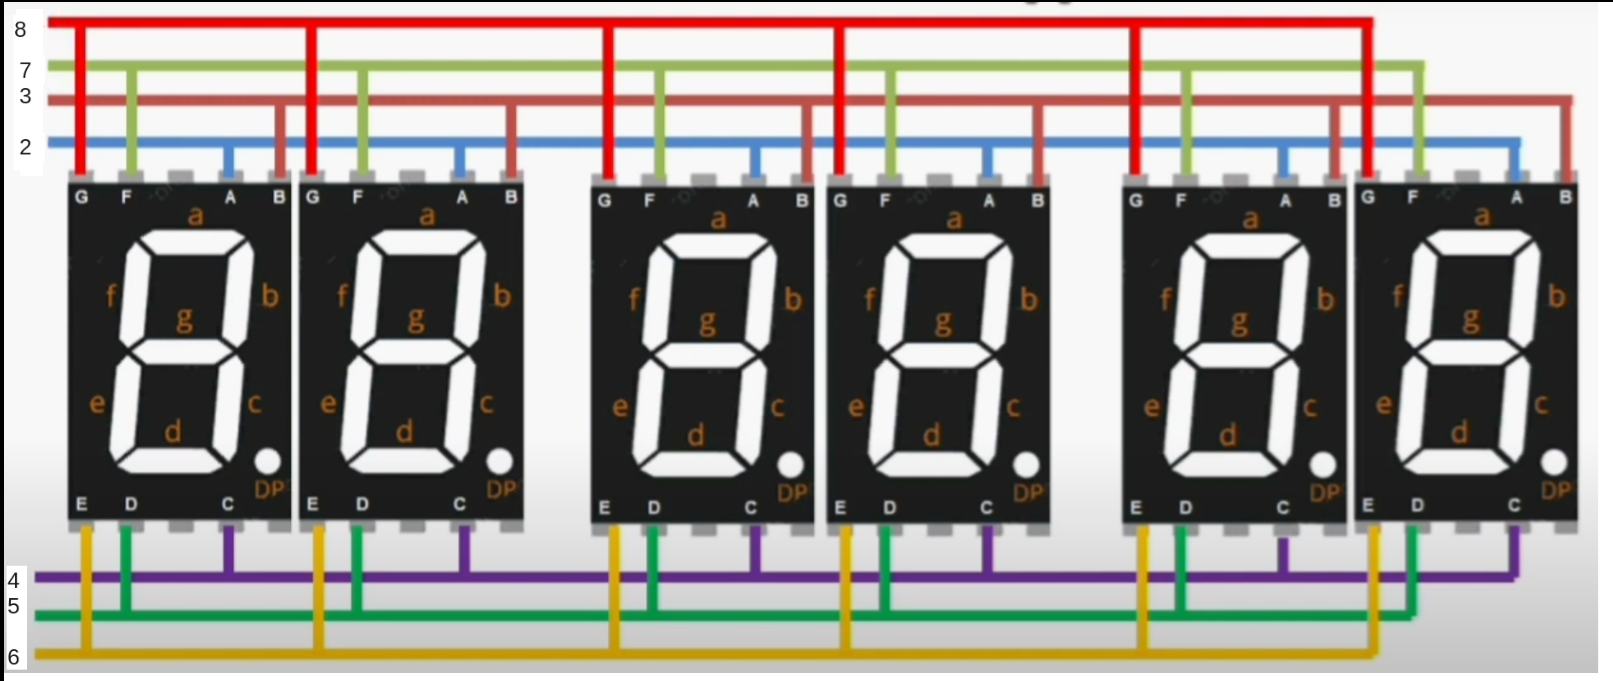
\includegraphics[width=0.75\columnwidth]{Connections/Connections.png}
\end{center}
\begin{itemize}
    \item The pins of seven segment display, Namely, a,b,c,d,e,f,g, are connected together.These are then connected to 2,3,4,5,6,7,8 pins on the arduino.
    \item The pin between a and f is COM(Common pin) of first display is connected to pin 9 on arduino.Similarly 2nd,3rd,4th,5th,6th COM pins are connected to 10,11,12,13,A0 pins on the arduino.
    \item The must be a resistor of \SI{220}{\ohm} between the COM pin and arduino pins to avoid high voltage which may  burn out the segments, making them dim permanently or stop working entirely.
    \item The dot pins are grounded.
\end{itemize}

\section{Working Principle-Software Implementation}

\subsection{Multiplexing}
\begin{enumerate}
    \item Multiplexing is a technique used to control multiple seven-segment displays using fewer Arduino pins by turning on one display at a time very quickly.
    \item This creates an illusion that all displays are ON simultaneously.
    \item All A-G segment pins of the displays are connected together and controlled by the same Arduino pins.
    \item The Arduino activates one display, sends the digit data, then quickly switches to the next display.
    \item The Arduino rapidly cycles through each display thousands of times per second, making it appear that all are ON at the same time.
\end{enumerate}

\subsection{Buttons Functionality}
\begin{enumerate}
    \item Initially we connect jumper wires to the analog pins (A1, A2, and A3).
    \item A1 controls the hour's units place (h2), A2 controls the minute's units place (m2), and A3 controls the second's units place (s2).
    \item We use a method called state change detection to capture when the jumper wire is connected (from HIGH to LOW) to increment the respective value (h2, m2, or s2).
    \item When the jumper wire is tapped on A1 (for example), the program checks if the current value of h2 (the hour's units place) is less than 9. If it is, the value increments by one.
    \item Similarly, tapping A2 increments the minutes' units place (m2), and A3 increments the seconds' units place (s2).
\end{enumerate}

\subsection{Debouncing}
\begin{enumerate}
    \item Mechanical buttons often generate noisy signals, causing bouncing, where the button state might change rapidly due to physical contact. This can cause multiple increments instead of just one.
    \item To prevent this, a debounce delay is added, which ensures that only one increment happens for each button press (or jumper wire tap).
    \item After detecting a state change, the program waits for a short period (e.g., 300 ms) before checking the button state again.
    \item This debounce delay helps ignore any unintended multiple presses from the same action.
\end{enumerate}

\subsection{Alarm functioning}
\begin{enumerate}
    \item We use analog pin A4 as the alarm setting button.
    \item When 4th Push button is pressed, the clock changes to alarm mode and we can use Hour pin, Minutes pin and seconds pin to set the alarm time.
    \item After setting the alarm time we again need to press A4 to fix the alarm time.
    \item Whenever the time is reached the buzzer rings for 15 seconds and goes off.
\end{enumerate}
\newpage
The following code is used to program the Arduino for controlling the digital clock. It handles multiplexing of six seven-segment displays, updates the time, allows us to set alarm and manages display refreshing.\\
\subsection{C Code}
\begin{small}
    
\begin{lstlisting}[language=C, breaklines=true, basicstyle=\ttfamily\footnotesize]

#include <avr/io.h>
#include <util/delay.h>
#include <avr/interrupt.h>
#include <stdint.h>

#define PINS_COUNT 6
#define NO_SEGMENTS 7

//Initialising the clock
uint8_t h1 = 0, h2 = 0, m1 = 0, m2 = 0, s1 = 0, s2 = 0;
uint8_t alarm_h1 = 0, alarm_h2 = 0, alarm_m1 = 0, alarm_m2 = 0, alarm_s1 = 0, alarm_s2 = 0;
uint8_t alarm_set = 0, alarm_active = 0, setting_alarm = 0;

#define HOUR_PIN PC1
#define MINUTE_PIN PC2
#define SECOND_PIN PC3
#define ALARM_PIN PC4
#define BUZZER_PIN PC5

volatile unsigned long millis_counter = 0;
uint8_t currentDisplay = 0;
unsigned long lastHourPress = 0, lastMinutePress = 0, lastSecondPress = 0, lastAlarmPress = 0;
unsigned long alarm_start_time = 0;

void timer0_init(void) {
    TCCR0A = 0;
    TCCR0B = (1 << CS01) | (1 << CS00);
    TIMSK0 = (1 << TOIE0);
    sei();
}

ISR(TIMER0_OVF_vect) {
    millis_counter += 1;
}

unsigned long millis(void) {
    return millis_counter;
}

void clearSegments(void) {
    PORTD &= 0b00000011;
    PORTB &= 0b11111110;
}

//Defining the connections of seven segment display to arduino
void sevenseg(uint8_t a, uint8_t b, uint8_t c, uint8_t d, uint8_t e, uint8_t f, uint8_t g) {
    clearSegments();
    PORTD |= (a << PD2) | (b << PD3) | (c << PD4) | (d << PD5) | (e << PD6) | (f << PD7);
    if (g) PORTB |= (1 << PB0); else PORTB &= ~(1 << PB0);
}

//Boolean logic for each segment of seven segment display
void segments(uint8_t A,uint8_t B, uint8_t C, uint8_t D){
	uint8_t a=!(A || C || (!B && !D) || (B && D));
	uint8_t b=!(A || (C && D) || !B ||(!C && !D));
	uint8_t c=!(A || B || !C || D);
	uint8_t d=!(A || ( C && !D) || (!B && !D ) || (!B && C) || (B && !C && D));
	uint8_t e=!((C && !D) || (!B && !D ));
	uint8_t f=!(A || (B && !C) || (B && !D ) || (!C && !D));
	uint8_t g=!((C && !D) || (!C && B) || (C && !B) || A);
	sevenseg(a, b, c, d, e, f, g);
}

//BCD for digits 0 to 9
void displayDigit(uint8_t digit) {
    static const uint8_t segment_map[10][4] = {
        {0, 0, 0, 0},
        {0, 0, 0, 1},
        {0, 0, 1, 0},
        {0, 0, 1, 1},
        {0, 1, 0, 0},
        {0, 1, 0, 1},
        {0, 1, 1, 0},
        {0, 1, 1, 1},
        {1, 0, 0, 0},
        {1, 0, 0, 1}
    };
     segments(segment_map[digit][0], segment_map[digit][1], segment_map[digit][2], segment_map[digit][3]);
}

//Function to display time
void displayClock(void) {
    PORTB &= 0b11000001;
    PORTC &= ~(1 << PC0);

    if (currentDisplay == 5) {
        PORTC |= (1 << PC0);
    } else {
        PORTB |= (1 << (currentDisplay + 1));
    }

    uint8_t display_val = (setting_alarm)
                              ? (currentDisplay == 0 ? alarm_h1 : currentDisplay == 1 ? alarm_h2
    : currentDisplay == 2 ? alarm_m1
    : currentDisplay == 3 ? alarm_m2
    : currentDisplay == 4 ? alarm_s1
    : alarm_s2)
    : (currentDisplay == 0 ? h1 : currentDisplay == 1 ? h2
    : currentDisplay == 2 ? m1
    : currentDisplay == 3 ? m2
    : currentDisplay == 4 ? s1
    : s2);

    displayDigit(display_val);
    currentDisplay = (currentDisplay + 1) % PINS_COUNT;
}

//Function to handle Hour button, Minute button ans seconds button
void handleButtons(void) {
    unsigned long currentMillis = millis();

    // Toggle alarm setting mode
    if (!(PINC & (1 << ALARM_PIN))) {
        if (currentMillis - lastAlarmPress > 300) {
            lastAlarmPress = currentMillis;
            setting_alarm = !setting_alarm;
            if (!setting_alarm) {
                alarm_set = 1;
            }
        }
    }

    // Adjust hours
    if (!(PINC & (1 << HOUR_PIN))) {
        if (currentMillis - lastHourPress > 300) {
            lastHourPress = currentMillis;
            uint8_t *h1_ptr = setting_alarm ? &alarm_h1 : &h1;
            uint8_t *h2_ptr = setting_alarm ? &alarm_h2 : &h2;

            (*h2_ptr)++;
            if (*h2_ptr >= 10) {
                *h2_ptr = 0;
                (*h1_ptr)++;
            }
            if (*h1_ptr >= 2 && *h2_ptr >= 4) {
                *h1_ptr = 0;
                *h2_ptr = 0;
            }
        }
    }

    // Adjust minutes
    if (!(PINC & (1 << MINUTE_PIN))) {
        if (currentMillis - lastMinutePress > 300) {
            lastMinutePress = currentMillis;
            uint8_t *m1_ptr = setting_alarm ? &alarm_m1 : &m1;
            uint8_t *m2_ptr = setting_alarm ? &alarm_m2 : &m2;

            (*m2_ptr)++;
            if (*m2_ptr >= 10) {
                *m2_ptr = 0;
                (*m1_ptr)++;
            }
            if (*m1_ptr >= 6) {
                *m1_ptr = 0;
            }
        }
    }

    // Adjust seconds
    if (!(PINC & (1 << SECOND_PIN))) {
        if (currentMillis - lastSecondPress > 300) {
            lastSecondPress = currentMillis;
            uint8_t *s1_ptr = setting_alarm ? &alarm_s1 : &s1;
            uint8_t *s2_ptr = setting_alarm ? &alarm_s2 : &s2;

            (*s2_ptr)++;
            if (*s2_ptr >= 10) {
                *s2_ptr = 0;
                (*s1_ptr)++;
            }
            if (*s1_ptr >= 6) {
                *s1_ptr = 0;
            }
        }
    }
}

//Function to check the alarm and activate the buzzer for 15 seconds
void checkAlarm(void) {
    static unsigned long last_toggle_time = 0;
    static uint8_t buzzer_state = 0;

    if (alarm_set && h1 == alarm_h1 && h2 == alarm_h2 && m1 == alarm_m1 && m2 == alarm_m2 && s1 == alarm_s1 && s2 == alarm_s2) {
        alarm_active = 1;
        alarm_start_time = millis();
    }

    if (alarm_active) {
        if (millis() - alarm_start_time < 15000) {
            if (millis() - last_toggle_time > 500) {
                last_toggle_time = millis();
                buzzer_state = !buzzer_state;
                if (buzzer_state) {
                    PORTC |= (1 << BUZZER_PIN);
                } else {
                    PORTC &= ~(1 << BUZZER_PIN);
                }
            }
        } else {
            alarm_active = 0;
            PORTC &= ~(1 << BUZZER_PIN);
        }
    }
}

//Function to update seconds minutes and hours in the clock
void updateClock(void) {
    static unsigned long lastUpdate = 0;
    if (millis() - lastUpdate >= 1000) {
        lastUpdate = millis();
        s2++;
        if (s2 >= 10) { s2 = 0; s1++; }
        if (s1 >= 6) { s1 = 0; m2++; }
        if (m2 >= 10) { m2 = 0; m1++; }
        if (m1 >= 6) { m1 = 0; h2++; }
        if (h2 >= 10) { h2 = 0; h1++; }
        if (h1 == 2 && h2 == 4) { h1 = 0; h2 = 0; }
        checkAlarm();
    }
}

int main(void) {
    DDRD |= 0b11111100;
    DDRB |= 0b00111111;
    DDRC |= (1 << PC0) | (1 << BUZZER_PIN);
    PORTC |= (1 << HOUR_PIN) | (1 << MINUTE_PIN) | (1 << SECOND_PIN) | (1 << ALARM_PIN);

    timer0_init();

    while (1) {
        updateClock();
        handleButtons();
        displayClock();
        _delay_ms(2);
    }
}


\end{lstlisting}
\end{small}

\section{Advantages of AVR-GCC}
\begin{itemize}
    \item Direct access to AVR registers which results in smaller and faster machine code.
    \item No C++ overhead (such as classes, virtual functions, and dynamic memory allocation).
    \item We can directly manipulate registers (e.g., PORTB, DDRC) for faster execution.
    \item No need for functions like digitalWrite(), which are slower than direct register access.
    \item No unnecessary code from high-level abstractions or unused libraries.
    \item Avoids unexpected behavior caused by library overhead.
    \item AVR-GCC is faster, more efficient, and gives complete hardware control. 
\end{itemize}

\section{Precautions}
\subsection{Hardware}
\begin{enumerate}
    \item  Always connect \SI{220}{\ohm} resistors in series with the seven-segment display segments to prevent excessive current draw and potential damage to the Arduino.
    \item  Double-check wiring to ensure no accidental short circuits, which could damage the microcontroller or display.
    \item  Before making any changes to the circuit, disconnect the Arduino from the power source to prevent accidental damage.
    \item Also connect a 1 Mega ohm Resistor in parallel to buzzer because buzzer can retain charge due to their internal capacitance.
    \item This can cause the buzzer to not turn off immediately or produce unwanted noise after switching off.
    \item A \SI{1}{M\ohm} resistor in parallel provides a path for residual charge to dissipate, ensuring the buzzer turns off completely after 15 seconds.
\end{enumerate}

\subsection{Software}
\begin{enumerate}
    \item  Ensure that the delay in the multiplexing loop is optimized to avoid flickering or unreadable digits. A 1.5-5ms delay per digit works well.
    \item Before uploading the code, double-check that the correct pins are assigned to the display segments and common anodes.
\end{enumerate}
\end{document}

